\documentclass[a4paper,10pt,english]{article}
\usepackage{%
	amsfonts,%
	amsmath,%	
	etex,%
	amssymb,%
	amsthm,%
	babel,%
	bbm,%
	%biblatex,%
	caption,%
	centernot,%
	color,%
	enumerate,%
	epsfig,%
	epstopdf,%
	geometry,%
	graphicx,%
	hyperref,%
	latexsym,%
	mathtools,%
	multicol,%
	pgf,%
	pgfplots,%
	pgfplotstable,%
	pgfpages,%
	proof,%
	psfrag,%
	subfigure,%	
	tikz,%
	ulem,%
	url%
}	

\usepackage[mathscr]{eucal}
\usepgflibrary{shapes}
\usetikzlibrary{%
  arrows,%
	backgrounds,%
	chains,%
	decorations.pathmorphing,% /pgf/decoration/random steps | erste Graphik
	decorations.text,%
	matrix,%
  	positioning,% wg. " of "
  	fit,%
	patterns,%
  	petri,%
	plotmarks,%
  	scopes,%
	shadows,%
  	shapes.misc,% wg. rounded rectangle
  	shapes.arrows,%
	shapes.callouts,%
  	shapes%
}

\theoremstyle{plain}
\newtheorem{thm}{Theorem}[section]
\newtheorem{lem}[thm]{Lemma}
\newtheorem{prop}[thm]{Proposition}
\newtheorem{cor}[thm]{Corollary}

\theoremstyle{definition}
\newtheorem{defn}[thm]{Definition}
\newtheorem{conj}[thm]{Conjecture}
\newtheorem{exmp}[thm]{Example}
\newtheorem{assum}[thm]{Assumptions}
\newtheorem{axiom}[thm]{Axiom}

\theoremstyle{remark}
\newtheorem{rem}{Remark}
\newtheorem{note}{Note}

\newcommand{\norm}[1]{\left\lVert#1\right\rVert}
\newcommand{\indep}{\!\perp\!\!\!\perp}
\DeclarePairedDelimiter\abs{\lvert}{\rvert}%
%\DeclarePairedDelimiter\norm{\lVert}{\rVert}%
\newcommand{\tr}{\operatorname{tr}}
\newcommand{\R}{\mathbb{R}}
\newcommand{\Q}{\mathbb{Q}}
\newcommand{\N}{\mathbb{N}}
\newcommand{\E}{\mathbb{E}}
\newcommand{\Z}{\mathbb{Z}}
\newcommand{\B}{\mathscr{B}}
\newcommand{\C}{\mathcal{C}}
\newcommand{\T}{\mathscr{T}}
\newcommand{\F}{\mathcal{F}}
\newcommand{\G}{\mathcal{G}}
%\newcommand{\ba}{\begin{align*}}
%\newcommand{\ea}{\end{align*}}

\makeatletter
\def\th@plain{%
  \thm@notefont{}% same as heading font
  \itshape % body font
}
\def\th@definition{%
  \thm@notefont{}% same as heading font
  \normalfont % body font
}
\makeatother
\date{}
%opening
\title{Lecture 13: Foster-Lyapunov Theorem}
\date{}%01 Mar 2016}
\author{}

\begin{document}
\maketitle
\section{Foster's Theorem}
\begin{thm}[Foster,1950]
Let $\{X_n\}_{n \geq 0}$ be a irreducible DTMC on $\mathbb{N}_0$ if there exist a function $L : \mathbb{N}_0 \longrightarrow \mathbb{R}_+$ with $\mathbb{E}[L(X_0)] < \infty$, such that for some $K>k\geq0$, and $\epsilon>0$:
\begin{enumerate}
\item $|\{x \in \mathbb{N}_0 : L(x) \leq k\}| < \infty$
\item $\mathbb{E}[L(X_n)|X_{n-1}] < K$,when $L(X_{n-1}) \leq k$.
\item $\mathbb{E}[L(X_n)-L(X_{n-1})|X_{n-1}] < -\epsilon$ if $L(X_{n-1})\geq k$
\end{enumerate}
Then $\{X_n\}_{n \geq 0}$ is positive recurrent.(L $\equiv$ "potential function" or energy or lyapunov function).
\end{thm}
\begin{proof}
As DTMC is irreducible than enough to show that some state is positive recurrent.
By renewal theory, for any DTMC, for all $x \in \mathbb{N}_0$,
\begin{align}
\lim\limits_{N \rightarrow \infty} \mathbb{E}\Big[ \sum_{n=1}^{N} \boldsymbol{1}_{\{X_n=x\}} \Big] = \frac{1}{\mu _{xx}} 
\end{align}
where 
\begin{equation*}
\mu _{xx}=
\begin{cases}
	\infty \ \ \ \ \ \ \ \ \ \ \ \ \ \ \ \ \ \ \ if \ $x$ \ is \ transient\\
	\sum_{m \geq 0}m f^{m}_{xx} \ \ \ \ \ \ \ \ if \ $x$ \ is \ recurrent \\
\end{cases}
\end{equation*}
consider the RHS of equation $(1)$
\begin{align*}
\lim\limits_{N \rightarrow \infty} \mathbb{E}\Big[ \sum_{n=1}^{N} \boldsymbol{1}_{\{X_n=x\}} \Big] > 0 \Longleftrightarrow x \ is \ positive \ recurrent  
\end{align*}
consider
\begin{align*}
& 0 \leq \mathbb{E}[L(X_n)] = \mathbb{E}[L(X_0)] +   \sum_{n=1}^{N}\mathbb{E}[L(X_n)-L(X_{n-1})]\\
&= \mathbb{E}[L(X_0)] + \sum_{n=1}^{N}\mathbb{E}[L(X_n)-L(X_{n-1})]\boldsymbol{1}_{\{L(X_{n-1})>k\}} + \sum_{n=1}^{N}\mathbb{E}[L(X_n)-L(X_{n-1})]\boldsymbol{1}_{\{L(X_{n-1})\leq k\}}\\
&\leq \mathbb{E}[L(X_0)] + \sum_{n=1}^{N}\mathbb{E}[-\epsilon \        \boldsymbol{1}_{\{L(X_{n-1})>k\}}] + \sum_{n=1}^{N}\mathbb{E}[K \ \boldsymbol{1}_{\{L(X_{n-1})\leq k\}}]\\
&\Rightarrow \Bigg[\mathbb{E}\sum_{n=1}^{N} \boldsymbol{1}_{\{L(X_{n-1})\leq k\}}\Bigg](K + \epsilon) \geq -\mathbb{E}[L(X_0)] + \epsilon N\\\\
&\Rightarrow \frac{1}{N} \Bigg[\mathbb{E}\sum_{n=1}^{N} \boldsymbol{1}_{\{L(X_{n-1})\leq k\}}\Bigg] \geq -\frac{\mathbb{E}[L(X_0)]}{N(K+\epsilon)} + \frac{\epsilon}{K+\epsilon}\\\\
&\Rightarrow \limsup_{N\rightarrow \infty}\frac{1}{N} \Bigg[\mathbb{E}\sum_{n=1}^{N} \boldsymbol{1}_{\{L(X_{n-1})\leq k\}}\Bigg] \geq \frac{\epsilon}{K+\epsilon}
\end{align*}
Let $F = \{x \in \mathbb{N}_0: L(x) \leq k\}, \ |F| < \infty$. Now,
\begin{align*}
& \limsup_{N\rightarrow \infty}\frac{1}{N} \Bigg[\mathbb{E}\sum_{n=1}^{N} \boldsymbol{1}_{\{L(X_{n-1})\leq k\}}\Bigg]\\\\
&=\limsup_{N\rightarrow \infty}\frac{1}{N} \Bigg[\mathbb{E}\sum_{n=1}^{N}\sum_{x \in F} \boldsymbol{1}_{\{X_{n-1}\leq k\}}\Bigg] \leq \sum_{x \in F} \Bigg[ \limsup_{N\rightarrow \infty}\frac{1}{N} \mathbb{E}\sum_{n=1}^{N} \boldsymbol{1}_{\{X_{n-1}\leq k\}}\Bigg]\\\\ 
&=\sum_{x \in F} \Bigg[ \limsup_{N\rightarrow \infty}\frac{1}{N} \mathbb{E}\sum_{n=1}^{N} \boldsymbol{1}_{\{X_{n-1}\leq k\}}\Bigg] \geq \frac{\epsilon}{K+\epsilon}>0
\end{align*}
Therefore there exist some $x \in F$ such that ,
\[\limsup_{N\rightarrow \infty}\frac{1}{N} \mathbb{E}\Bigg[ \sum_{n=1}^{N} \boldsymbol{1}_{\{X_{n-1}\leq k\}}\Bigg] \geq \frac{\epsilon}{(K+\epsilon)|F|}>0\]\\\\
Therefore there exist some $x \in F$ such that ,
\[\lim_{N\rightarrow \infty}\frac{1}{N} \mathbb{E}\Bigg[\sum_{n=1}^{N} \boldsymbol{1}_{\{X_{n-1}\leq k\}}\Bigg] >0\]
\end{proof}
\section{Applications of Foster's theorem: Queue scheduling/Max-weight scheduling}
Consider $N$ queue served by a single server in discrete time(Figure 1).
At time slot t = 1,2,3....\\
$A_i(t) \in \mathbb{N}_0$ packets arrive to each queue $i \in [N]$ independently.\\
\begin{figure}
\centering
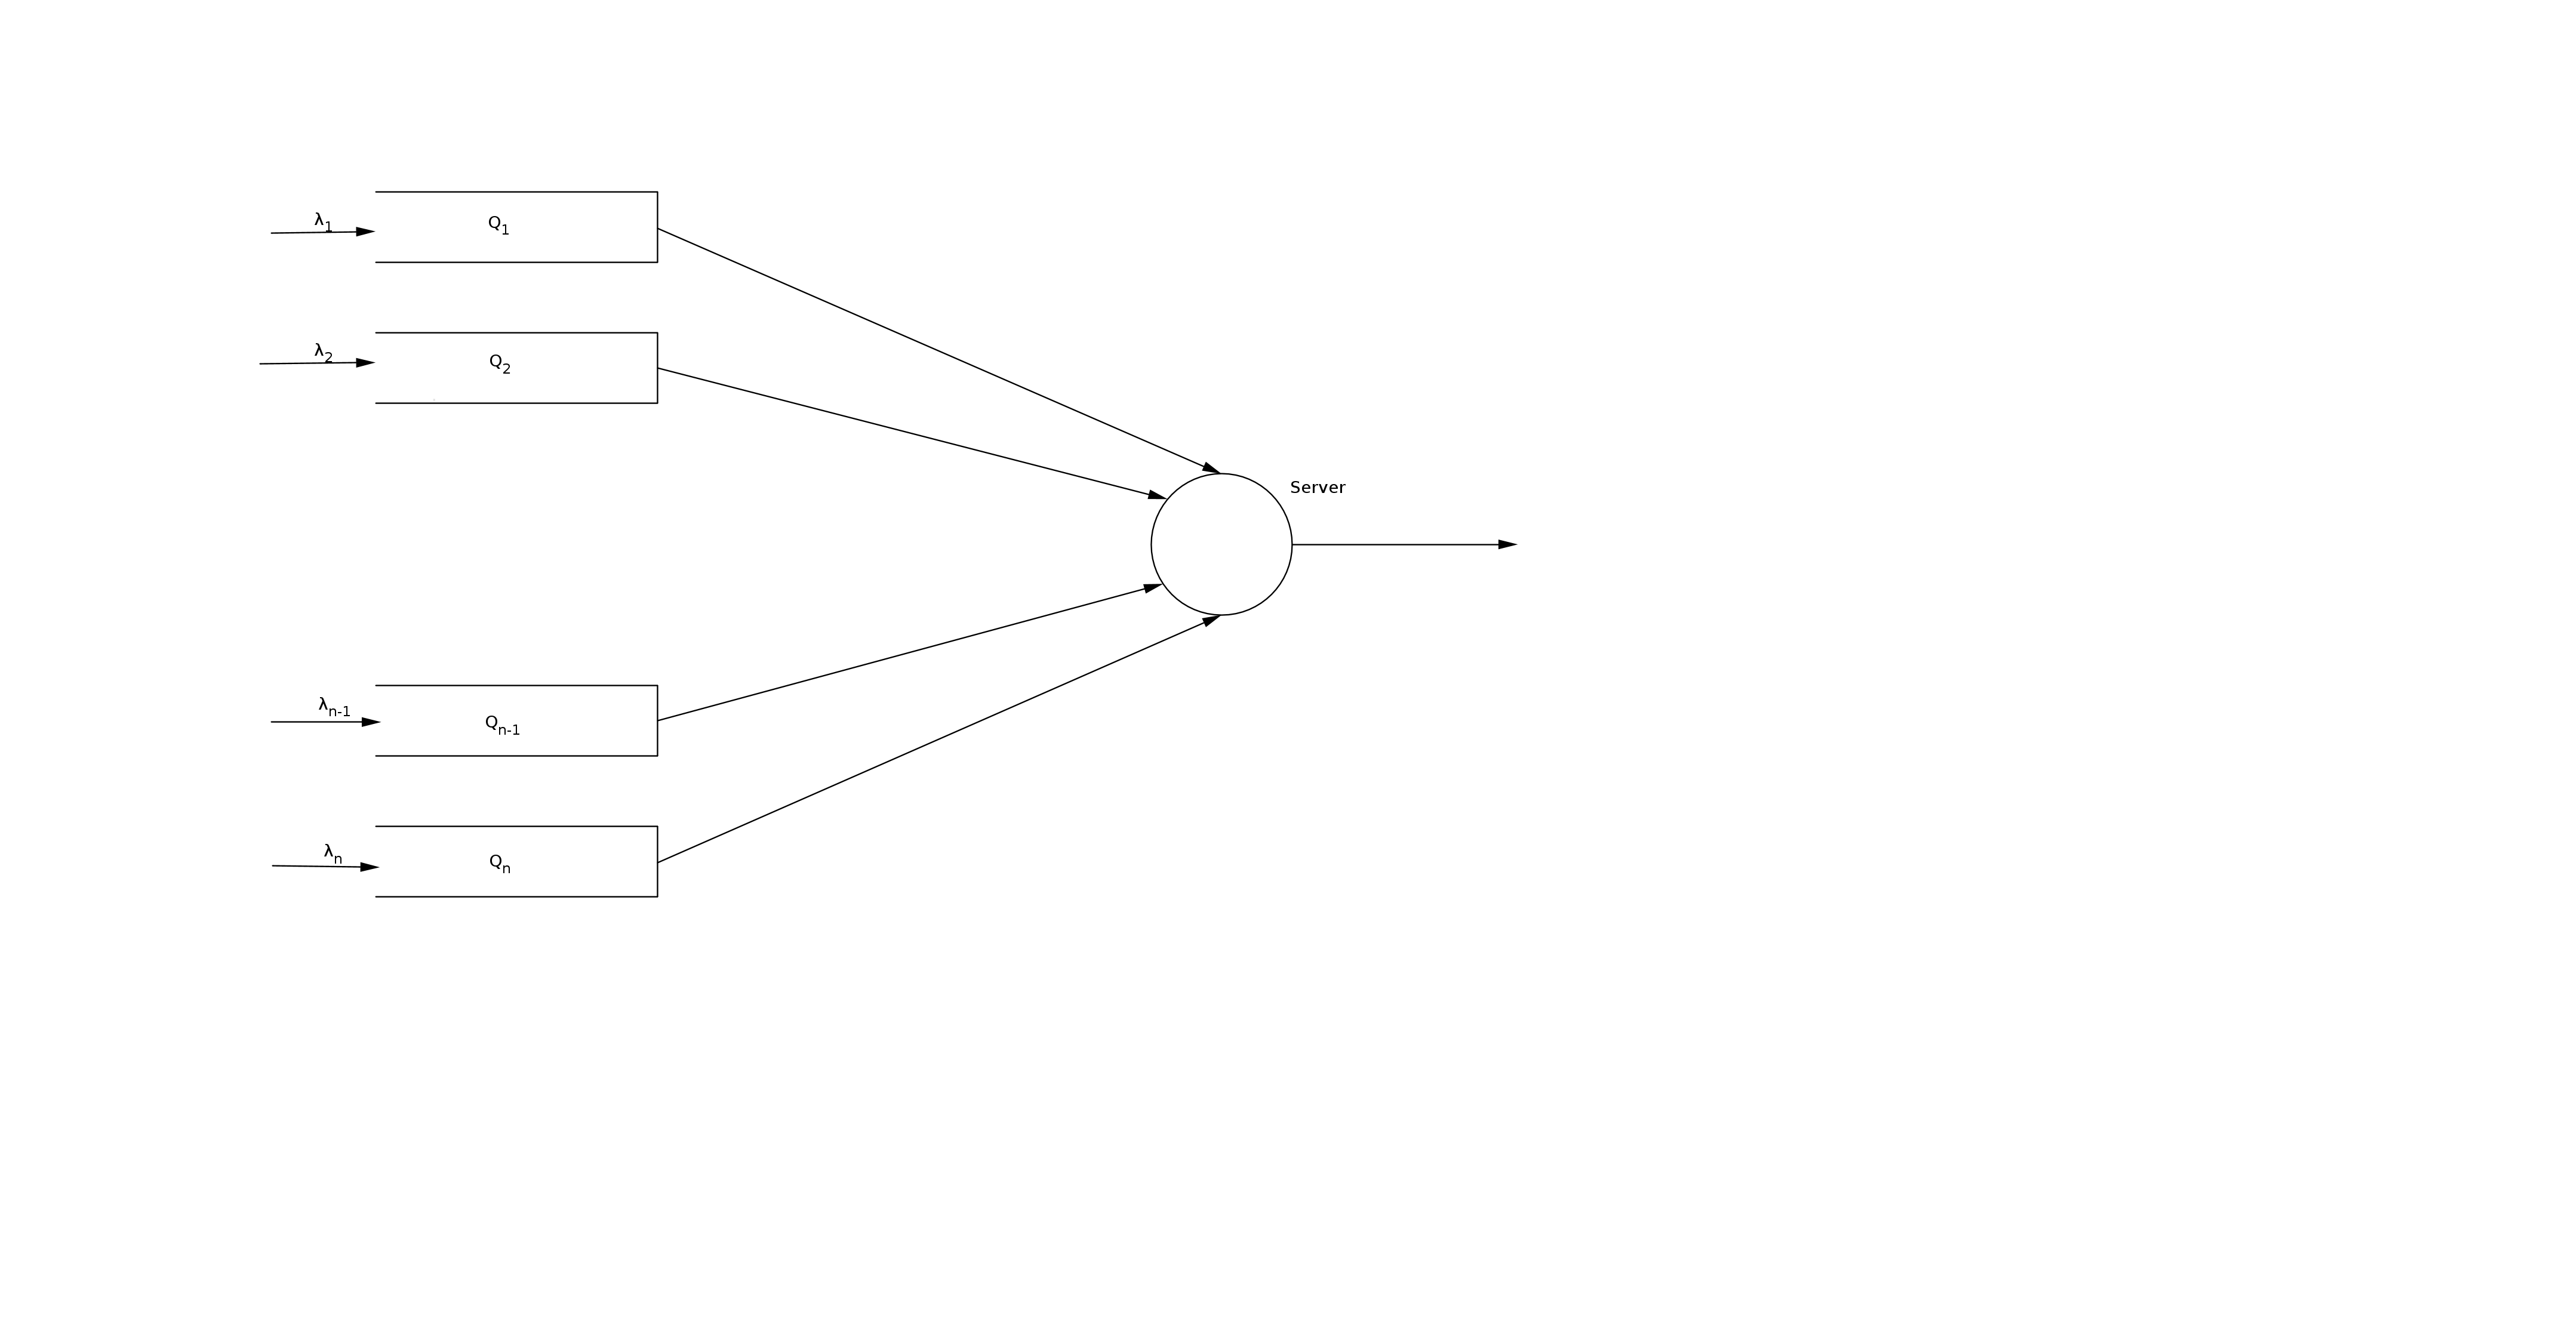
\includegraphics[scale=0.6]{Figures/saa.png}
\caption{N queues single server, server chooses one queue and serve upto one packet}
\label{fig: example 1.1}
\end{figure}
\begin{enumerate}
\item $\mathbb{E}[A_i(t)] = \lambda _i$
\item $\mathbb{P}[A_i(t)=0] > 0$
\item $\mathbb{E}[A_i(t)^2] \leq C$
\end{enumerate}
Server picks one queue $Q(t) \in [N]$ for service. Let $R_i(t) =  \boldsymbol{1}\{Q(t) = i\}$.One packet is served from $Q(t)$ if it is not empty.Let $X_i(t)$ = number of packets in queue $i$ just before time slot $t$.\\
\[X_i(t+1) = (X_i(t) + A_i(t) - R_i(t))_+\]
Where \[a_+ = max(0,a)\]
aslo \[X_i(t+1) = X_i(t) + A_i(t) - R_i(t) + L_i(t)       \]Where 
\begin{equation*}
L_i(t) = 
\begin{cases}
  1 \ \ \ \,service \ attempted \ when \ i \ is \ empty\\
  0 \ \ \ \,otherwise 
\end{cases}
\end{equation*}
Mean rate of arrivals to system : $= \sum_{i=1}^{N} \lambda _i
$\\
Maximum rate of departure $= 1$, we will assume $ \sum_{i=1}^{N} \lambda _i < 1$.
\begin{thm}[Max-weight scheduling algorithm, 1992]
\[Q(t) = \arg \max _{i \in N} X_i(t)  \] 
that is serve  the longest queue.Under MAX-WT ,$X(t) = (X_i(t))_{i=1}^{N}$ is a DTMC which is irreducible and aperiodic on state space $\mathbb{N}_0^N$.As long as $\sum_{i=1}^{N} \lambda _i < 1$, $\{X_n\}$ is positive recurrent.
\end{thm}
\begin{proof}
By Foster's theorem, define the Lyapunov function:
\[L(x) = \frac{1}{2} \sum_{i=1}^{N}x_i^2\] consider
\begin{align*}
& L(X(t)) - L(X(t-1))\\
&= \frac{1}{2} \sum_{i=1}^{N}\Big[ (X_i(t))^2 - (X_i(t-1))^2 \Big]\\
&= \frac{1}{2} \sum_{i=1}^{N}\Big[ \{X_i(t-1) + A_i(t-1) - R_i(t-1) + L_i(t-1)\}^2 - (X_i(t-1))^2 \Big]\\
& \leq \frac{1}{2} \sum_{i=1}^{N}\Big[ \{X_i(t-1) + A_i(t-1) - R_i(t-1)\}^2 - (X_i(t-1))^2 \Big]
\end{align*}
Therefore 
\[\mathbb{E}\Big[ L(X(t)) - L(X(t-1)) | X(t-1) = x \Big]  \leq \frac{1}{2} \sum_{i=1}^{N} \mathbb{E} \Big[ (x_i + A_i(t-1) - R_i(t-1))^2 - x_i^2 | X(t-1) = x \Big]\]
\begin{align*}
&= \frac{1}{2} \sum_{i=1}^{N} \Bigg[ 2x_i \mathbb{E} \Big[ (A_i(t-1) - R_i(t-1)| X(t-1) = x \Big] + \mathbb{E} \Big[ (A_i(t-1) - R_i(t-1))^2 | X(t-1) = x \Big] \Bigg]\\
&= \sum_{i=1}^{N}x_i \lambda _i - \sum_{i=1}^{N}x_i R_i(t-1) + \frac{N}{2}(1+C)\\
&= \sum_{i=1}^{N}x_i \lambda _i + \frac{N}{2}(1+C) - \max _i x_i\\
& \leq \frac{N}{2}(1+C) + (\max _i x_i)(\sum_{i=1}^{N} \lambda _i - 1)\\
&= C_1 - \epsilon (\max _i x_i)
\end{align*}
Foster's theorem applies with $k = \max \{\frac{\|x\|_2 ^2}{2}\}$
\end{proof}
\end{document}

